\chapter{Architecture Générale du Système}

\section{Vue d'ensemble}

L'architecture retenue pour ce projet est basée sur une approche \textbf{défense en profondeur} (\textit{defense in depth}) : chaque couche de l'écosystème dispose de ses propres mécanismes de sécurité, de sorte qu'une compromission partielle ne compromet pas l'ensemble du système.

\begin{figure}[H]
  \centering
  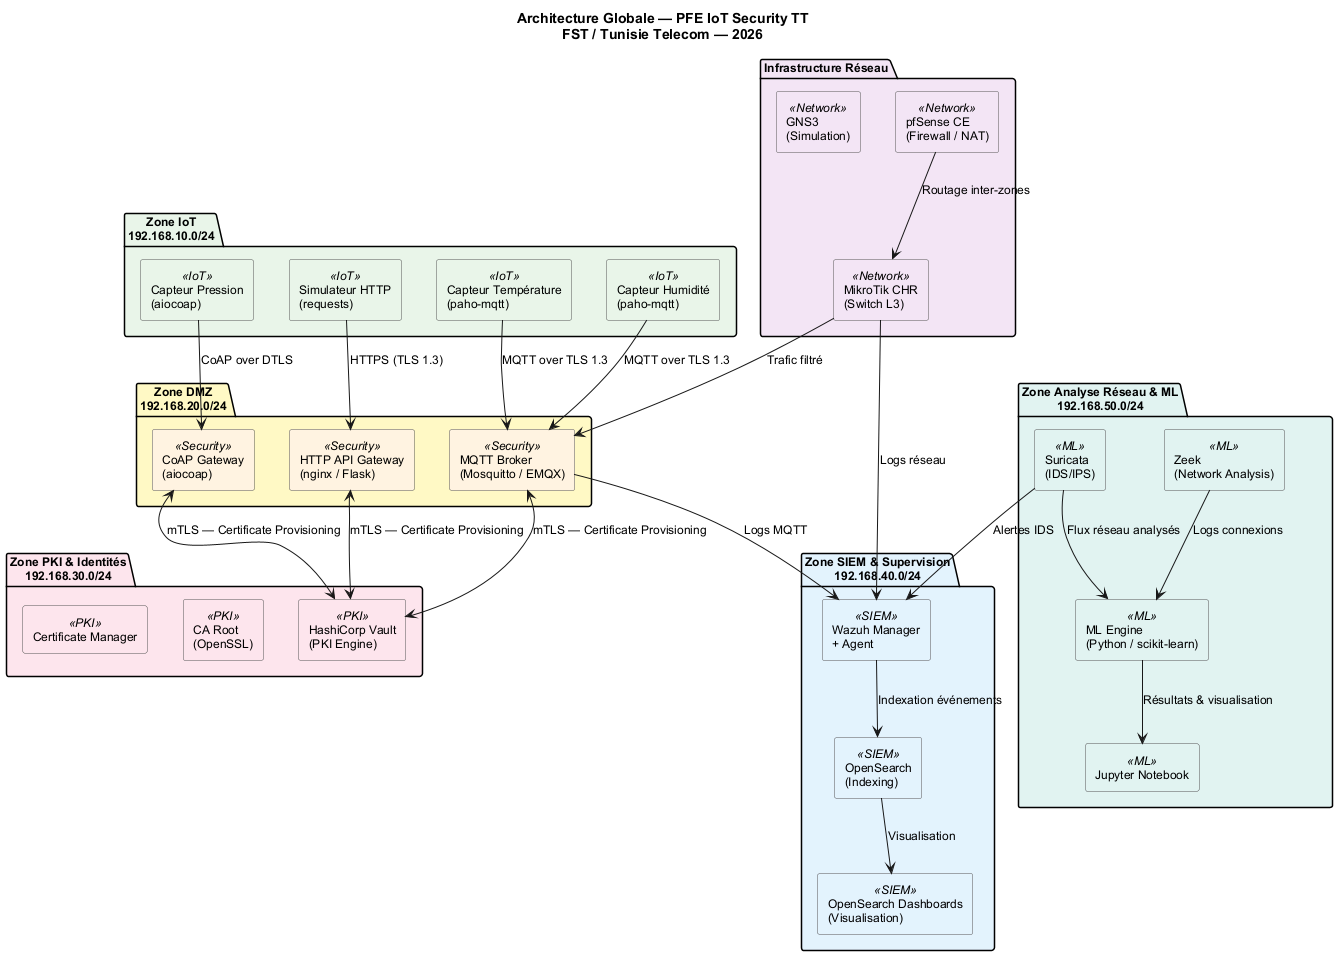
\includegraphics[width=\textwidth]{figures/architecture-generale.png}
  \caption{Architecture générale de l'écosystème IoT sécurisé}
  \label{fig:archi_generale}
\end{figure}

\section{Topologie réseau GNS3}

La simulation réseau est réalisée sous \textbf{GNS3} (Graphical Network Simulator 3) avec VMware Workstation Pro comme hyperviseur. L'environnement comprend :

\subsection{Segmentation réseau}

\begin{table}[H]
\centering
\caption{Plan d'adressage de la topologie GNS3}
\label{tab:adressage}
\begin{tabular}{lllp{5cm}}
\toprule
\textbf{Réseau} & \textbf{CIDR} & \textbf{Composants} & \textbf{Rôle} \\
\midrule
IoT Devices & 192.168.10.0/24 & fleet-simulator, capteurs & Zone devices — trafic MQTT non chiffré interne \\
Services & 192.168.20.0/24 & Mosquitto, Vault, Suricata & Zone services sécurisés \\
Management & 192.168.30.0/24 & Wazuh OVA & Zone administration et SIEM \\
\bottomrule
\end{tabular}
\end{table}

\subsection{Composants réseau}

Un routeur \textbf{MikroTik CHR} (RouterOS v7) assure le routage inter-VLAN et implémente les règles de pare-feu (firewall) :
\begin{itemize}
  \item Autorisation explicite du port 8883 (MQTT/TLS) de la zone IoT vers la zone Services.
  \item Blocage de tout trafic direct IoT $\to$ Management.
  \item NAT masquerade pour l'accès Internet (mises à jour, time sync).
\end{itemize}

\begin{figure}[H]
  \centering
  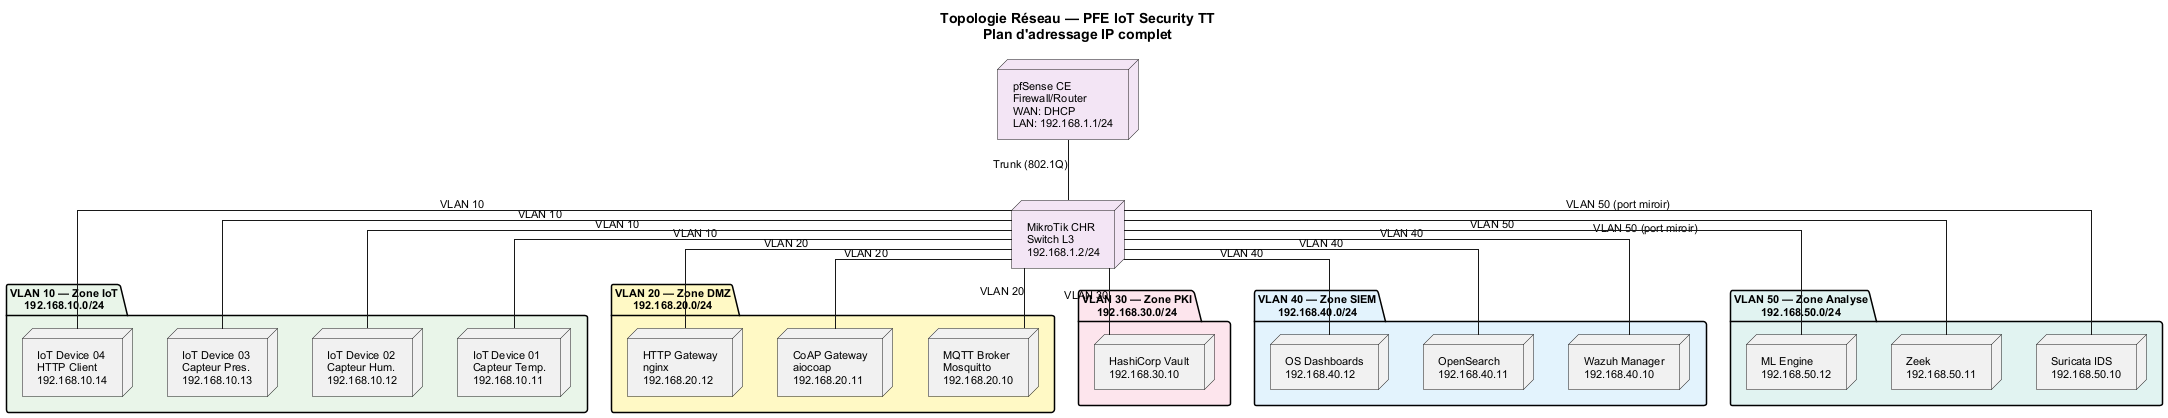
\includegraphics[width=\textwidth]{figures/gns3-topology.png}
  \caption{Topologie réseau dans GNS3}
  \label{fig:gns3_topology}
\end{figure}

\section{Composants applicatifs}

\subsection{Broker MQTT — Mosquitto}

Eclipse Mosquitto v2.0 est déployé en conteneur Docker sur la zone Services (192.168.20.10). Il est configuré avec :
\begin{itemize}
  \item TLS 1.3 strict (port 8883 uniquement, port 1883 désactivé).
  \item mTLS obligatoire (\texttt{require\_certificate true}).
  \item ACL basée sur le \textbf{Common Name} du certificat client.
\end{itemize}

\subsection{PKI — HashiCorp Vault}

Vault v1.15 est déployé sur 192.168.20.20. Il héberge :
\begin{itemize}
  \item Un moteur PKI racine (\texttt{pki}) avec une CA hors-ligne simulée.
  \item Un moteur PKI intermédiaire (\texttt{pki\_int}) émettant les certificats de services et de dispositifs.
  \item Des politiques Vault contrôlant l'accès à l'API d'émission de certificats.
\end{itemize}

\subsection{Fleet Simulator}

Le simulateur de flotte est un conteneur Python (192.168.10.X) rejouant le dataset CSV de 76\,000 événements. Chaque dispositif simulé possède un certificat unique émis par Vault.

\subsection{Suricata IDS}

Suricata v7.0 est déployé en mode \textit{AF\_PACKET} sur le segment Services, avec une copie du trafic réseau via un switch GNS3 en mode hub.

\subsection{Wazuh SIEM}

Wazuh v4.7 est déployé sous forme d'OVA VMware sur 192.168.30.128. Il ingère :
\begin{itemize}
  \item Les alertes Suricata (\texttt{/var/log/suricata/eve.json}).
  \item Les logs du broker Mosquitto.
  \item Les journaux système des conteneurs.
\end{itemize}

\section{Flux de données E2E sécurisé}

Le flux de communication de bout en bout suit les étapes suivantes :

\begin{enumerate}
  \item Le dispositif IoT demande un certificat à Vault via l'API REST (authentification par token).
  \item Vault émet un certificat X.509 signé par la CA intermédiaire, valide 24 heures.
  \item Le dispositif établit une connexion TLS 1.3 avec Mosquitto (port 8883), en présentant son certificat.
  \item Mosquitto valide la chaîne de certification et autorise la connexion si le CN correspond à la politique ACL.
  \item Les messages MQTT sont publiés sur les topics autorisés et transités vers les subscribers.
  \item Suricata inspecte le trafic réseau et génère des alertes JSON dans \texttt{eve.json}.
  \item Wazuh ingère les alertes Suricata et les corrèle avec d'autres événements.
  \item Le pipeline ML analyse les métriques de communication pour détecter des anomalies.
\end{enumerate}

\section{Choix technologiques}

Les principaux choix techniques ont été motivés par les critères suivants :

\begin{table}[H]
\centering
\caption{Justification des choix technologiques}
\label{tab:choix_tech}
\begin{tabular}{llp{6cm}}
\toprule
\textbf{Composant} & \textbf{Technologie} & \textbf{Justification} \\
\midrule
Simulation réseau & GNS3 & Standard académique, support Docker natif, reproductible \\
Routeur & MikroTik CHR & Utilisé en production chez TT, RouterOS complet \\
Broker MQTT & Mosquitto & Open-source, TLS 1.3 natif, ACL avancées, communauté active \\
PKI & HashiCorp Vault & API programmatique, rotation automatique, open-source \\
IDS & Suricata & Support MQTT natif, multi-thread, règles compatibles Snort \\
SIEM & Wazuh & OpenSearch intégré, agents légers, gratuit et open-source \\
ML & scikit-learn & Large écosystème, IsolationForest + RF disponibles \\
\bottomrule
\end{tabular}
\end{table}
